\documentclass[10pt]{beamer}
\usepackage{tikz}
\usepackage{pgfplots}
\usepackage{mathtools}
\usepackage{physics}
\usepackage{amsfonts,amsmath,amssymb,amsthm}
\usetikzlibrary{shapes.geometric, arrows}

\tikzstyle{startstop} = [rectangle, rounded corners, minimum width=3cm, minimum height=1cm, text centered, draw=black, fill=red!30]
\tikzstyle{process} = [rectangle, minimum width=3cm, minimum height=1cm, text centered, draw=black, fill=blue!30]
\tikzstyle{decision} = [diamond, minimum width=3cm, minimum height=1cm, text centered, draw=black, fill=green!30]
\tikzstyle{arrow} = [thick,->,>=stealth]

\usetheme[progressbar=frametitle]{metropolis}
\usepackage{appendixnumberbeamer}

\usepackage{booktabs}

\usepackage{pgfplots}
\usepgfplotslibrary{dateplot}

\usepackage{xspace}
\newcommand{\themename}{\textbf{\textsc{metropolis}}\xspace}

\title{Adversarial Pheromone-based Swarm Robots Dynamics as System of Stochastic Partial Differential Equations}
%\subtitle{Case study: Information Operation}
% \date{\today}
\date{}
\author{Aukkawut Ammartayakun}
\institute{University of Tennessee, Knoxville}
% \titlegraphic{\hfill\includegraphics[height=1.5cm]{logo.pdf}}

\definecolor{utorange}{RGB}{255, 130, 0}
\setbeamercolor{frametitle}{bg=utorange, fg=white}
\setbeamercolor{background canvas}{bg=white}
\begin{document}

\maketitle
\begin{frame}{Table of contents}
  \setbeamertemplate{section in toc}[sections numbered]
  \tableofcontents%[hideallsubsections]
\end{frame}
\section{Spatial-Temporal Influence Maximization in Swarm Robotics}
\begin{frame}{Pheromone-Based Robot Foraging}
\begin{figure}
    \centering
    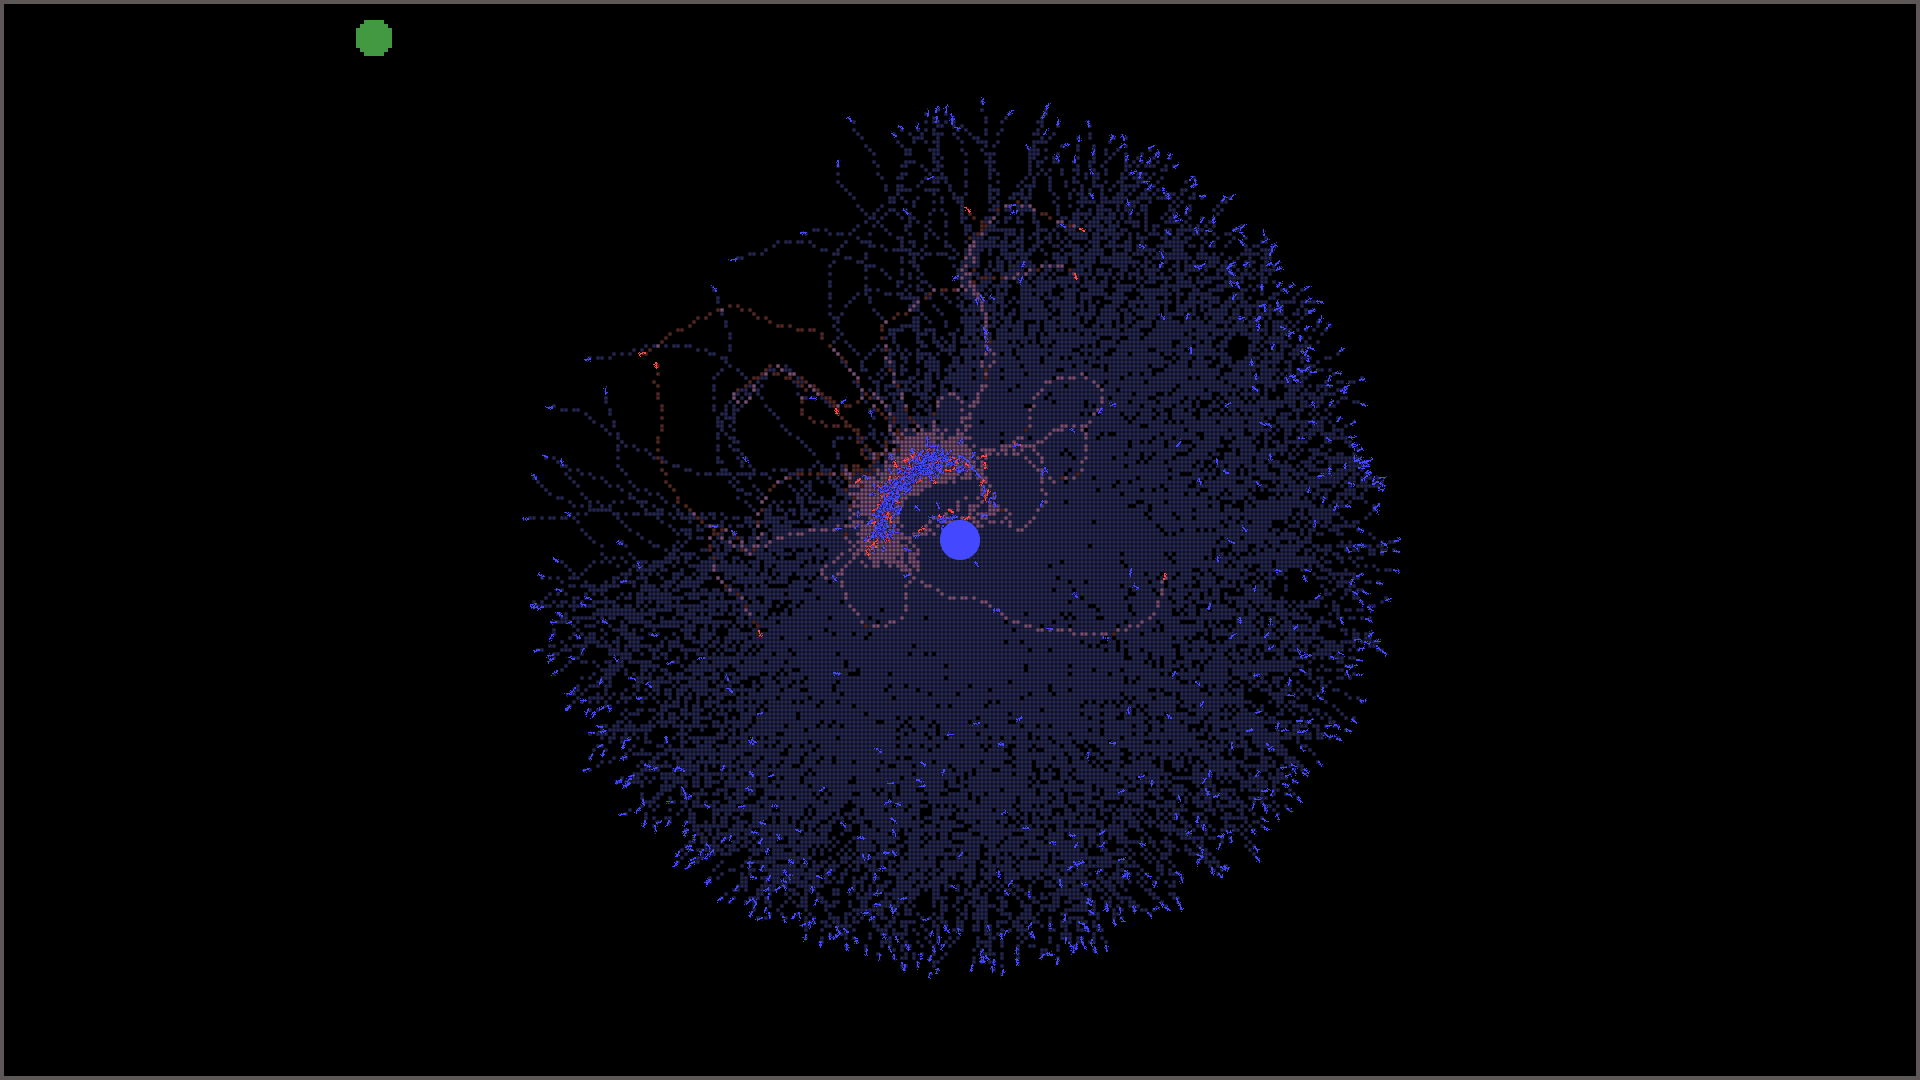
\includegraphics[width=1\linewidth]{DetractorWall.png}
    \caption{\textbf{Effect of Malicious Actor on the Foraging.} Green is food, blue circle is nest. Blue trails is to-food pheromone and red is adversarial to-food pheromone.}
    \label{fig:2}
\end{figure}
\end{frame}
\begin{frame}{Pheromone-Based Robot Foraging: Cautionary Pheromone}
\begin{figure}
    \centering
    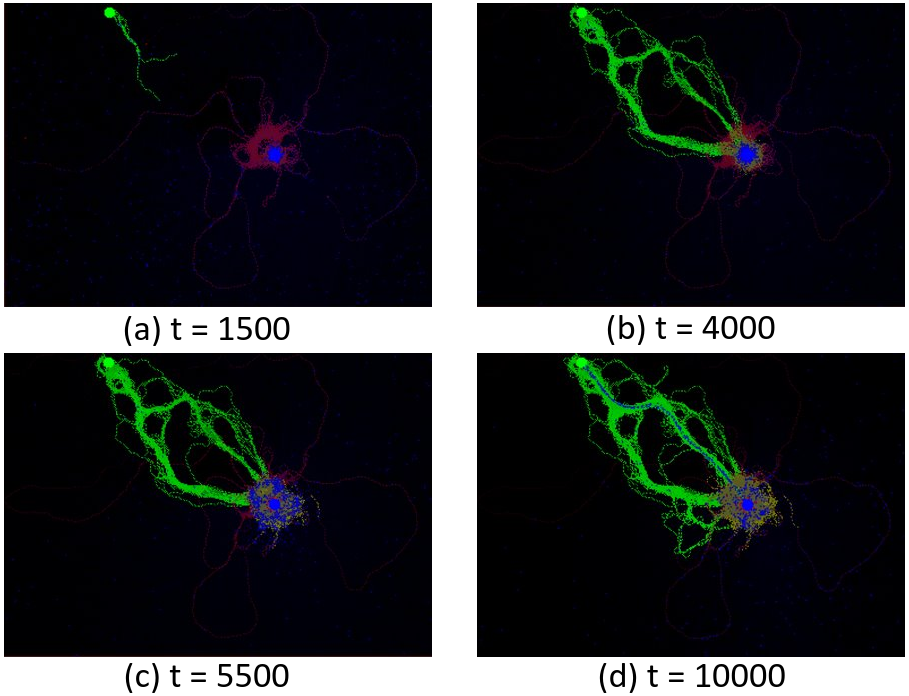
\includegraphics[width=0.8\linewidth]{counter_timeline.png}
    \caption{\textbf{Time Evolution Of Pheromone Concentration Given Cautionary Pheromone} (Aswale et al., AAMAS 2022)}
    \label{fig:2}
\end{figure}
\end{frame}
\section{Related Work}
\begin{frame}{Modeling Pheromone Coupled System}
    \begin{itemize}
        \item Bruna et al. (2025) uses Fokker-Planck and eliptical equation
        \begin{align*}
            \frac{\partial}{\partial t}f &= \nabla_x \cdot\left(D_T\nabla_x{f}-\eta\begin{bmatrix}\cos\theta\\ \sin\theta\end{bmatrix}f\right)+\frac{\partial}{\partial\theta}\left(\frac{\partial}{\partial\theta}f-\gamma B[c]f\right)\\
            \nabla^2c-\alpha c + \rho&=0\\
            B_\lambda[c] &= \begin{bmatrix}-\sin\theta\\ \cos\theta\end{bmatrix}\cdot\nabla_xc\left(x+\lambda \begin{bmatrix}\cos\theta\\ \sin\theta\end{bmatrix}\right)\\
            \underbrace{f(t=0,x,\theta)}_{\text{time,space,orientation}}&=f^{0}(x,\theta)
        \end{align*}
        \begin{itemize}
            \item Strong point for this model is well-posedness and interaction which can be used to model the robot.
            \item Weak point is that it doesn't follow gradient flow, hence is complicated to analyze.
        \end{itemize}
    \end{itemize}
\end{frame}
\begin{frame}{Adversarial Problems}
\begin{itemize}
    \item Aswale et al. (2022) proposes the framework and the empirical result of the adversarial pheromone robot problem. 
    \begin{itemize}
        \item The impact of the faulty/malicious robot is so great (in simulation), we only need tiny amount of the adversarial agents to disrupt the operation.
        \item They propose cautionary pheromone to ``erase" the malicious pheromone after some time.
    \end{itemize}
        \item Strobel et al. (2023) proposed token economy system to mitigate the effect of adversaries. 
    \begin{itemize}
        \item Requires token to act, resulting in adversaries depleting their tokens.
    \end{itemize}
\end{itemize}
    
\end{frame}

  \begin{frame}{Research Questions}
  \begin{itemize}
      \item What is optimal strategy or optimal dynamics $Y_t$ such that it minimize $F(t)$?
      \item Can we do anything against it without additional ``things"?
      \begin{itemize}
          \item Internal belief $p_i(t)$ $\implies$ Exploration-exploitation problem
          \item Treating adversarial pheromone as noise $\implies$ filtering problem?
          \item Clever information propagation?
      \end{itemize}
  \end{itemize}
  \end{frame}
\section{Theoretical Model}
\begin{frame}{Pheromone and Robot Dynamics}
\begin{itemize}
    \item Suppose $i=1,\dots,N$ are robots that locate at $x_i(t)$. At position $x(t)$, there are 2 pheromones concentration $P_\text{food},P_{\text{home}}$
    \[
    \dd x_i(t) = \overbrace{v_i(t) \dd t}^\text{correlated term} + \underbrace{\sigma \dd W_i(t)}_{\text{random walk}}
    \]
    \[
    \dfrac{\partial}{\partial t} P_\ell(x,t) = \overbrace{D_\ell \nabla^2P_\ell(x,t)}^{\text{diffusion}} - \underbrace{\lambda_\ell P_\ell(x,t)}_{\text{evaporation}} +\overbrace{S_\ell(x,t)}^{\text{deposition}}, \quad \ell\in\{\text{food},\text{home}\}
    \] (Ryan, Journal of Mathematical Biology, 2016)
    \item Note that pheromone dynamics is SPDE as \[S_\ell(x,t) = \sum_{i=1}^N s_i(t)\delta(x-X_i(t))\] for random position $X_i(t)$ described by dynamics $\dd x_i(t)$
    \item Robot has prior belief in trustworthiness of the observation.
\end{itemize}
\end{frame}
	\begin{frame}{Adversaries}
		\begin{itemize}
			\item Suppose the dynamics $X_i(t)$ is now defined as
				\[
				\dd X_i = \begin{cases}
				\mu(\nabla P) \dd t + \sigma \dd W_t & \text{ w.p. } p\\
				\sigma \dd W_t & \text{ w.p. } 1-p
				\end{cases}
				\]
			\item Now, we have hidden Bernoulli process.
      \item Goal: Represent $p$ with some dynamics
      \item Moreover, we can argue that there exists $\Lambda = \{\lambda_1,\dots,\lambda_m\}\subseteq \{1,\dots,N\}$ such that for any robot in $\Lambda$, the dynamics for random walk is diffrent compared to the rest of cohort (i.e, adversaries).

		\end{itemize}
	\end{frame}
  \begin{frame}{Model}
    \begin{itemize}
      \item WLOG, there are $N$ robots, $1,\dots, n$ are under normal operation, $n+1, \dots, N$ are faulty (or adversaries).
      \item System follows this dynamics
        \begin{align*}
          \dfrac{\partial}{\partial t} P(x,t) &= D\nabla^2 P(x,t) - \gamma P(x,t) + S_n(x,t)+ S_f(x,t)\\
          S_n(x,t) &= \sum_{i=1}^{n}s_n\delta(x-X_i(t))\\
          \dd X_i(t) &= Z_i(t)\left[\mu(\nabla P(X_i(t),t))\dd t + \sigma \dd W_t\right] + (1-Z_i(t))\sigma\dd W_t\\
          Z_i(t) &\sim \operatorname{Ber}(p(t))\\
          S_f(x,t) &= \sum_{k=n+1}^N s_f \delta(x-Y_k(t))\\
          \dd Y_k(t) &= \varphi(\nabla P(Y_k(t),t),t)\dd t + \eta \dd W_t
        \end{align*}
    \end{itemize}
  \end{frame}
  \begin{frame}{Model (continue)}
  \begin{itemize}
  \item What we don't know
        \begin{itemize}
          \item $n$, how many adversaries.
          \item $Y_k(t)$ dynamics of adversaries.
        \end{itemize}
  \item What we should assume
    \begin{itemize}
      \item Lipschitz (for existence of the solution of $P$)
      \item Covariance structure of $Z_i(t_1)$ and $Z_i(t_2)$ for $t_1\neq t_2$ (for Markovian)
    \end{itemize}
  \end{itemize}
  \end{frame}
  \begin{frame}{Cumulative Food}
    \begin{itemize}
      \item Now, the objective function for the robot is to maximize the cumulative food
      \begin{align*}
F(t) &= \sum_{i=1}^n \int_0^t \int_{\mathbb{R}^d} 1_{\{\text{carrying}_i(\tau)\}} \cdot \delta(X_i(\tau) - x_0) \cdot r(X_i(\tau^-), \tau) \, dx \, d\tau \\
r(x,t) &= \min\left(r_{\max}, \phi(x,t)\right) \\
\frac{\partial \phi(x,t)}{\partial t} &= - \sum_{i=1}^n \delta(x - X_i(t)) \cdot 1_{\{X_i(t) \in \mathcal{F}\}} \cdot r(x,t)
\end{align*}
\item Decision Variable: 
\begin{itemize}
    \item Adversaries: dynamics $Y_t$
    \item Non-adversaries: $p_i(t)$ or $X_t$
\end{itemize}
    \end{itemize}
  \end{frame}
  \begin{frame}{How to solve this?}
      \begin{itemize}
          \item Suppose we are considering this at discrete time and discrete space (grid world or lattice), then there are a lot of ways to work with this
          \begin{itemize}
              \item Similar manner to immersed boundary method (Peskin, 1972), we can propagate the ``fluid" on the ``field" and interact with ``solid".
              \item Or can model this as percolation problem (Grimmett, 1999).
              \item One of the adversarial strategy can be modeled as ``absorbing state" (Morimoto et al., 2025)
          \end{itemize}
          \item Incorporate the robot dynamics control into the model in orientation manner rather than pure spatial-temporal system (Malíčková et al. 2015; Bruna et al., 2025)
          \item Using mean-field theory to understand effect of local interaction (particles) to the global parameter (temperature) (Ornia et al. 2022; Morimoto et al., 2025)
      \end{itemize}
  \end{frame}
  


\end{document}
            
